\chapter{QCD}
\label{ch:qcd}

\MyQuote{Is the purpose of theoretical physics to be no more than a cataloging of all the
things that can happen when particles interact with each other and separate? Or
is it to be an understanding at a deeper level in which there are things that
are not directly observable (as the underlying quantized fields are) but in
terms of which we shall have a more fundamental understanding?}
{Julian Schwinger}

The theoretical framework of particle physics is called the Standard Model (SM). The
SM describes the way how the fundamental components of matter interact with each
other through strong, weak and electromagnetic interactions. Mathematically the
SM is a gauge quantum field theory with local internal symmetries of the direct
product group $SU(3) \times SU(2) \times U(1)$. Gauge bosons are assigned to
generators of this symmetry - there are 8 massless gluons from $SU(3)$ and 3
massive $W^\pm, Z$ bosons with 1 massless boson $\gamma$ from electroweak $SU(2)
\times U(1)$ sector. Higgs mechanism has to be introduced in the electroweak sector
to assign $W^\pm, Z$ bosons masses and as consequence the new particle - Higgs
boson - emerges in the SM theory. All bosons have integer spin. 

In addition to the bosons the SM introduces spin-1/2 fermions which are
divided into three quark and three lepton families. Fermions are assumed to be
point-like because there is no evidence for their internal structure to date.
All fermions interact weakly, if they have electrical charge, they interact
electromagnetically as well. Quarks are the only fundamental fermions which do
interact strongly. System of fundamental particles of the SM is shown in
Figure~\ref{fig:SMparticles}. 

\begin{figure}[!ht]
  \centering
  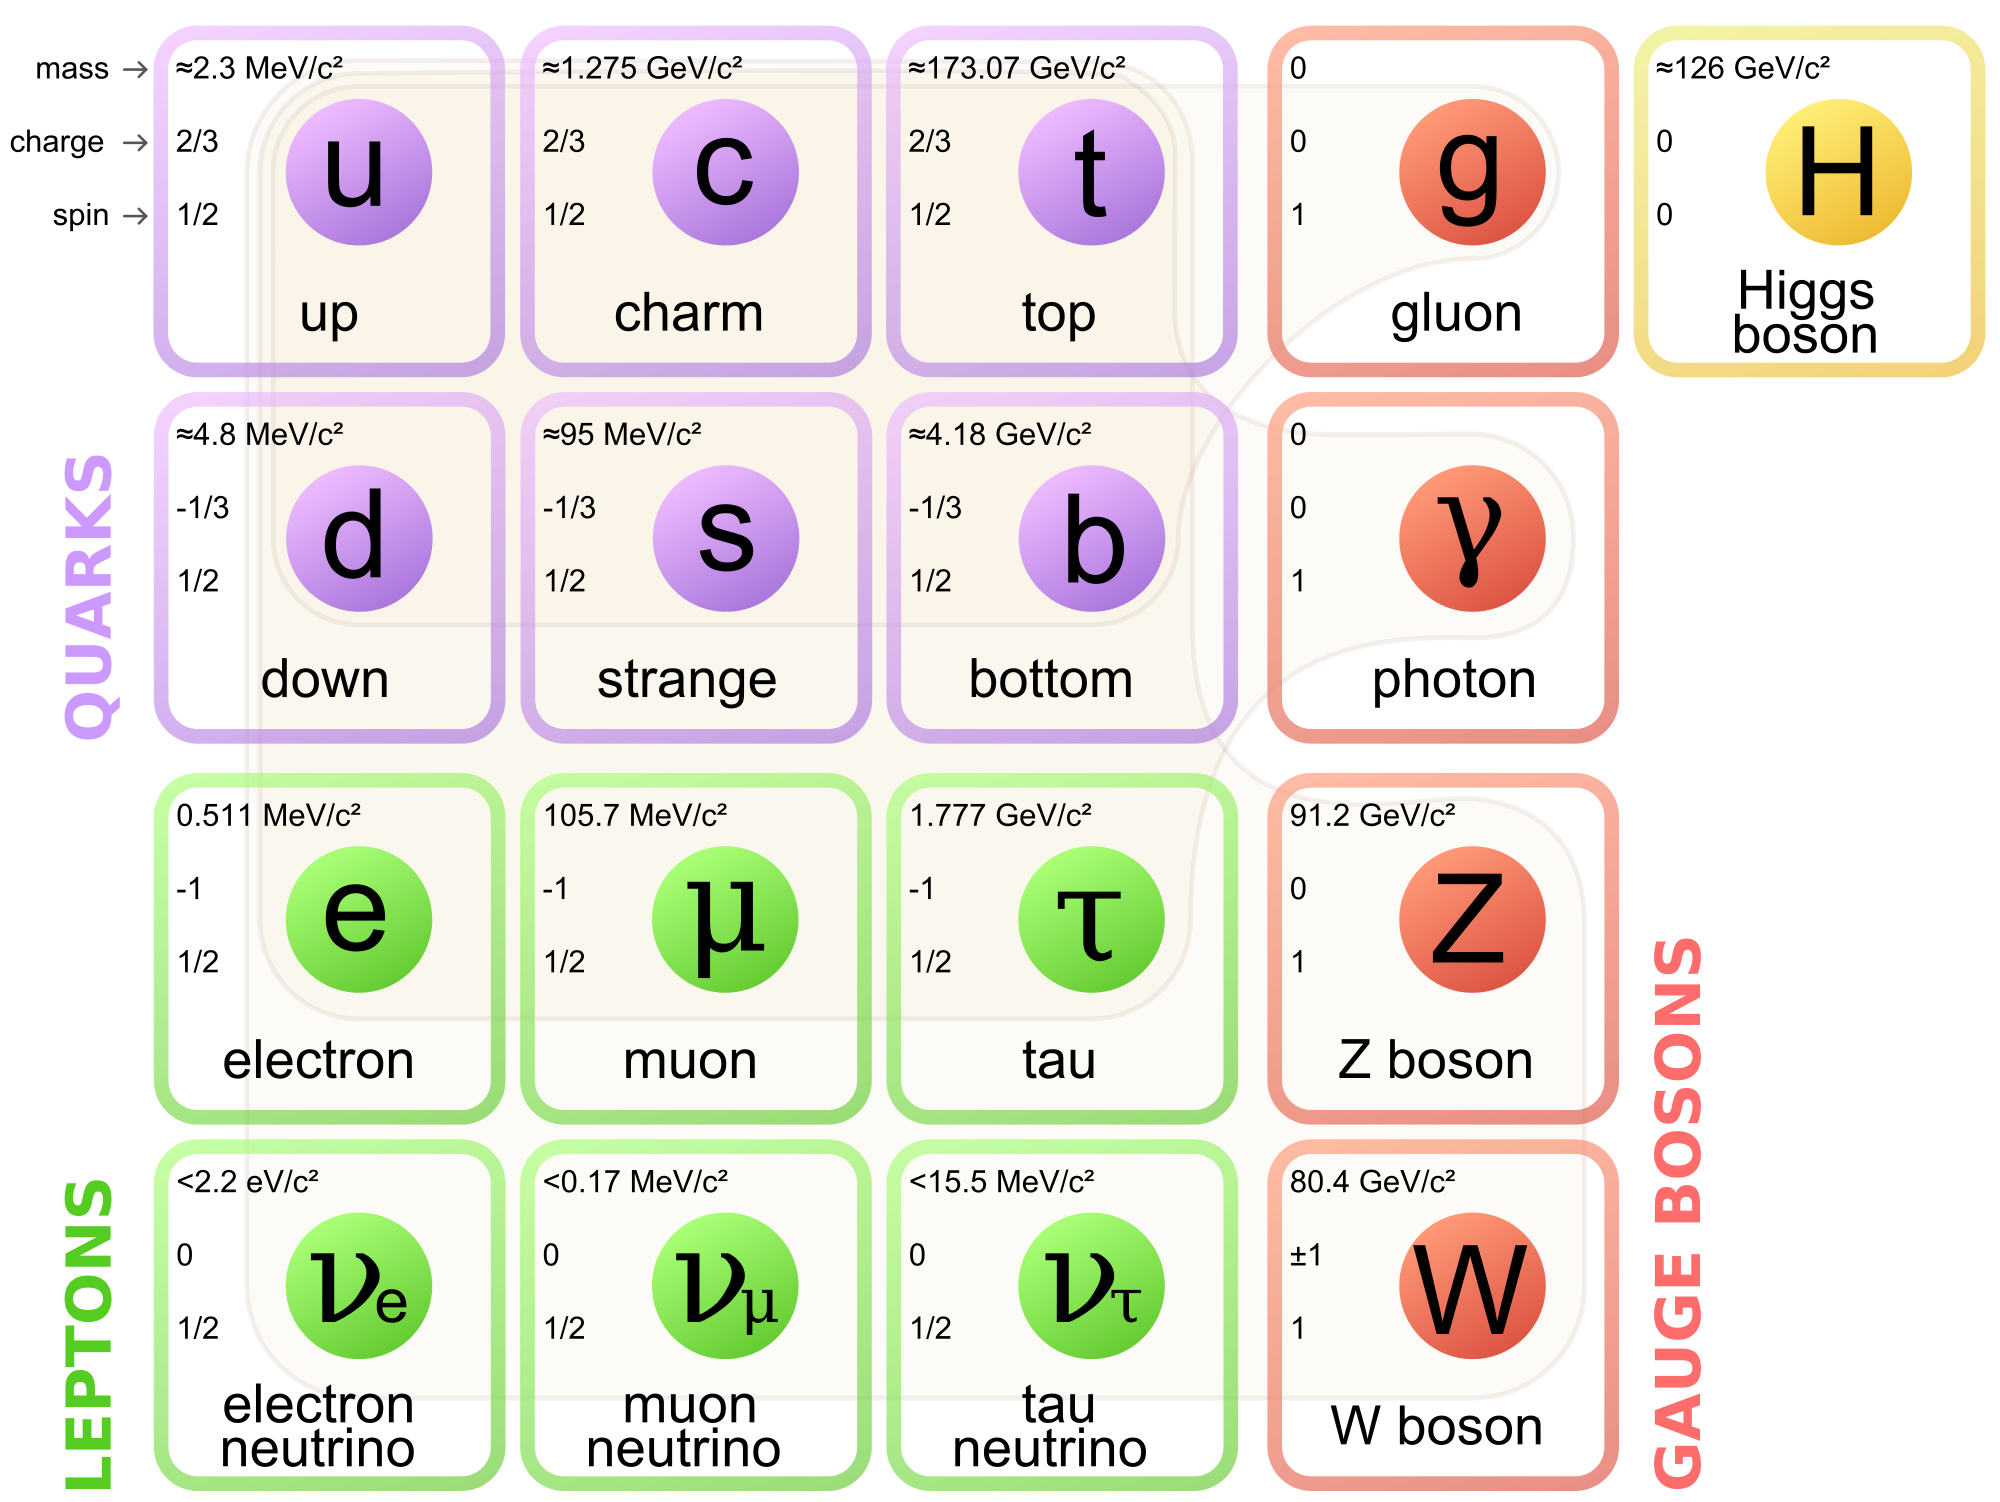
\includegraphics[width=\textwidth]{Chapter1/SM.png} 
  \caption{The system of fundamental particles of the SM. Figure from
    \cite{wiki:SMParticlesSource}.}
  \label{fig:SMparticles}
\end{figure}

Quarks bind together to form hadrons and there are hundreds
\cite{PDG2014} of known hadrons up to date. Hadrons are
divided into baryons (3 quarks) and mesons (quark and anti-quark pairs). Theory
describing the interaction between quarks is called Quantum Chromodynamics (QCD)
which key features will be discussed in this chapter. The reasoning for quark
existence and for the description their strong interaction as $SU(3)$ gauge
theory will be presented. Running coupling constant will be discussed to split
QCD into perturbative and non-perturbative regions - two regions, where QCD has
to use different mathematical approaches for the description of strong
interaction. Most of ideas presented here is overtaken from the following
textbook \cite{QCDTextbook}. Electroweak sector of the SM is described in
\cite{horejsi2002fundamentals}. For more concise information about the SM the
following textbooks can serve
\cite{griffiths2008introduction,cottingham2007introduction}.

\section{Theoretical Ansatz}
\label{Sec:TheoreticalAnsatz}

In 1950s, there have already been discovered tens of new hadrons thanks to new
particle accelerators and a lot of effort was exerted to categorize them. To each
particle there was assigned a series of quantum numbers
including isospin $T$ with its third component $T_3$, hypercharge $Y$,
electrical charge $Q$, strangeness $S$, baryon number $B$ and others. Soon it
was recognized, that there are some symmetries between these quantum numbers,
like famous Gell-Mann--Nishijima relation
\cite{GellMannNishijima1,GellMannNishijima2}

\begin{equation}
  Q = T_3 + 1/2 Y \quad , \quad Y = B + S + \dots,
  \label{ex:GellMannNishijima}
\end{equation}
where dots denote charm, bottomness and topness and were introduced after work
of Gell-Mann and Nishijima. Some of the baryons known by then are shown in
Table~\ref{tab:SelectedHadrons}. In 1960s, the known hadrons were successfully
categorized with the so called Eightfold Way, which was published independently
by Murray Gell-Mann \cite{Gell-Mann:101798} and George Zweig \cite{Zweig:570209}
in 1964. The Eightfold Way successfully predicted the existence of new particle
$\Omega^{-}$ including its mass. Basic ideas of Eightfold Way will be discussed
in this section.

\begin{table}
  \centering
  \begin{tabular}{|C{1cm}|C{1cm}|C{1cm}|C{1cm}|C{1cm}|C{1cm}|}
    \hline
     & $S$ & $Y$ & $T$ & $T_3$ & $Q$  \\
    \hline \hline
    $p$ & \multirow{2}{*}{0} & \multirow{2}{*}{1} & \multirow{2}{*}{1/2} & 1/2  & 1 \\
    $n$ &                    &                    &                      & -1/2 & 0 \\
    \hline                                                              
    $\Sigma^+$  & \multirow{4}{*}{-1} & \multirow{4}{*}{0} & \multirow{3}{*}{1} & 1  & 1  \\
    $\Sigma^0$  &                     &                    &                    & 0  & 0  \\
    $\Sigma^-$  &                     &                    &                    & -1 & -1 \\
    $\Lambda$   &                     &                    & 0                  & 0  & 0  \\
    \hline                                                              
    $\Xi^0$ & \multirow{2}{*}{-2} & \multirow{2}{*}{-1} & \multirow{2}{*}{1/2} & 1/2 & 0  \\
    $\Xi^-$ &                     &                     &                      &-1/2 & -1 \\
    \hline
  \end{tabular}
  \caption{Quantum numbers of selected baryons known in 1950s. $S$ strangeness,
  $Y$ hypercharge, $T$ isospin, $T_3$ third component of isospin, $Q$ electrical
charge.}
  \label{tab:SelectedHadrons}
\end{table}

The key feature of Eightfold Way is to understand hadrons as the part of
different representations of infinitesimal generators of $SU(3)$ flavor symmetry
group. These infinitesimal generators of $SU(3)$ form the real eight-dimensional
Lie algebra $\mathfrak{su}(3)$ which fundamental representation is usually
derived from Gell-Mann matrices

\begin{align}
  &\lambda_1 = \begin{pmatrix} 0 & 1 & 0 \\ 1 & 0 & 0 \\ 0 & 0 & 0 \end{pmatrix}
  \quad
  \lambda_2 = \begin{pmatrix} 0 & -i & 0 \\ i & 0 & 0 \\ 0 & 0 & 0 \end{pmatrix}
  \quad
  \lambda_3 = \begin{pmatrix} 1 & 0 & 0 \\ 0 & -1& 0 \\ 0 & 0 & 0 \end{pmatrix}
  \nonumber \\
  &\lambda_4 = \begin{pmatrix} 0 & 0 & 1 \\ 0 & 0 & 0 \\ 1 & 0 & 0 \end{pmatrix}
  \quad
  \lambda_5 = \begin{pmatrix} 0 & 0 & -i\\ 0 & 0 & 0 \\ i & 0 & 0 \end{pmatrix}
  \label{eq:GellMannMatrices} \\
  &\lambda_6 = \begin{pmatrix} 0 & 0 & 0 \\ 0 & 0 & 1 \\ 0 & 1 & 0 \end{pmatrix}
  \quad
  \lambda_7 = \begin{pmatrix} 0 & 0 & 0 \\ 0 & 0 & -i\\ 0 & i & 0 \end{pmatrix}
  \quad
  \lambda_8 = \frac{1}{\sqrt{3}} \begin{pmatrix} 1 & 0 & 0 \\ 0 & 1 & 0 \\ 
                                                              0 & 0 & -2 \end{pmatrix}.
  \nonumber
\end{align}

The generators are usually chosen $g_a = \frac{1}{2} \lambda_a$ and obey the
commutation relation $[g_a,g_b]=if_{abc}g_c$ with $f_{abc}$ being structure
constants. Cartan subalgebra of fundamental representation of $\mathfrak{su}(3)$
is generated by $H_1=g_3$ and $H_2=g_8$. The eigenstates of three-dimensional
representation of $\mathfrak{su}(3)$ can be chosen 

\begin{equation}
  u = \begin{pmatrix} 1 \\ 0 \\ 0 \end{pmatrix} \leftrightarrow \left(
    \frac{1}{2}, \frac{\sqrt{3}}{6} \right), \quad
  d = \begin{pmatrix} 0 \\ 1 \\ 0 \end{pmatrix} \leftrightarrow \left(
    - \frac{1}{2}, \frac{\sqrt{3}}{6} \right), \quad
  s = \begin{pmatrix} 0 \\ 0 \\ 1 \end{pmatrix} \leftrightarrow \left(
    0, - \frac{\sqrt{3}}{3} \right), \quad
  \label{eq:RepresentLie3}
\end{equation}
where the eigenvalues to generators of the Cartan subalgebra was assigned $H_1 u
= \frac{1}{2} u$, $H_2 u = \frac{\sqrt{3}}{6} u$ and similarly for $d$ and $s$
eigenstates. These eigenvalues are shown in Figure~\ref{fig:QuarkTriplet}. Other
important representation of $\mathfrak{su}(3)$ is eight-dimensional adjoint
representation. This representation has the following eigenstates and
corresponding eigenvalues

\begin{SCfigure}
  \centering
  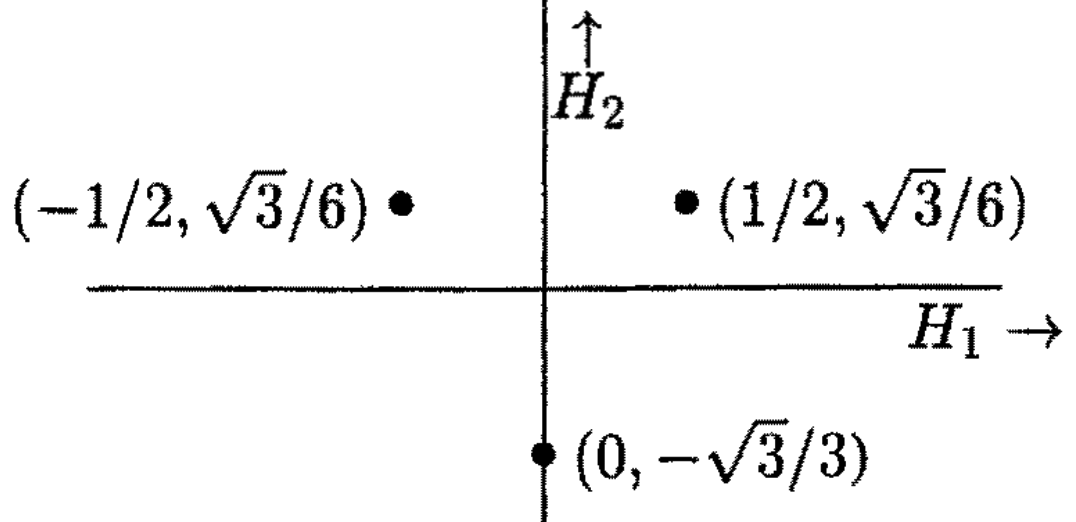
\includegraphics[width=0.5\textwidth]{Chapter1/Quark-triplet.png} 
  \caption{Eigenvalues of 3-dimensional representation of $\mathfrak{su}(3)$ Lie algebra. Figure
    from \cite{LieAlgebrasForParticlePhysicists}.}
  \label{fig:QuarkTriplet}
\end{SCfigure}

\begin{align}
  \frac{1}{\sqrt{2}} \left( g_1 \pm i g_2  \right)
    &\leftrightarrow \left( \pm 1, 0 \right), \nonumber \\
  \frac{1}{\sqrt{2}} \left( g_4 \pm i g_5 \right) 
    &\leftrightarrow \left( \pm \frac{1}{2}, \pm \frac{\sqrt{3}}{2} \right), 
    \label{eq:RepresentLie8} \\
  \frac{1}{\sqrt{2}} \left( g_6 \pm i g_7 \right) 
    &\leftrightarrow \left( \mp \frac{1}{2}, \pm \frac{\sqrt{3}}{2} \right), \nonumber
\end{align}
where again when denoting $A = \frac{1}{\sqrt{2}} ( g_1 + i g_2 )$ then the
upper sign of the first expression reads $[ H_1, A ] = A$ and $[ H_2, A ] = 0$ and
similarly for remaining 5 eigenstates. Defining 

\begin{equation}
  H_1 = T_3 \quad \text{and} \quad H_2 = \frac{\sqrt{3}}{2} Y
  \label{eq:LieIdentification}
\end{equation}
one can easily assign hadrons from table
\ref{tab:SelectedHadrons} to corresponding eigenvalues of adjoint
representation in \eqref{eq:RepresentLie8} according to its third component of
isospin $T_3$ and its hypercharge $Y$. This is depicted in
Figure~\ref{fig:BaryonicOctet}. 

When the same redefinition is done to the eigenstates
of three-dimensional representation in \eqref{eq:RepresentLie3}, one can assign to
eigenstates the hypercharge $Y$ and strangeness $S$ as well. The concrete values for
states $u$, $d$, $s$ are shown in Table~\ref{tab:SelectedQuarks}.

\begin{table}
  \centering
  \begin{tabular}{|C{1cm}|C{1cm}|C{1cm}|C{1cm}|C{1cm}|C{1cm}|}
    \hline
     & $S$ & $Y$ & $T$ & $T_3$ & $Q$  \\
    \hline \hline
    $u$ & \multirow{2}{*}{0} & \multirow{2}{*}{1/3} & \multirow{2}{*}{1/2} & 1/2
    & 2/3 \\
    $d$ &                    &                      &                      &
    -1/2 & \multirow{2}{*}{-1/3} \\
    $s$ & -1                 & -2/3                 & 0                    & 0    &  \\
    \hline                                                              
  \end{tabular}
  \caption{Quantum numbers of three quarks which existence was predicted by
    Gell-Mann and Zweig in 1964.}
  \label{tab:SelectedQuarks}
\end{table}

\begin{SCfigure}[][t]
  \centering
  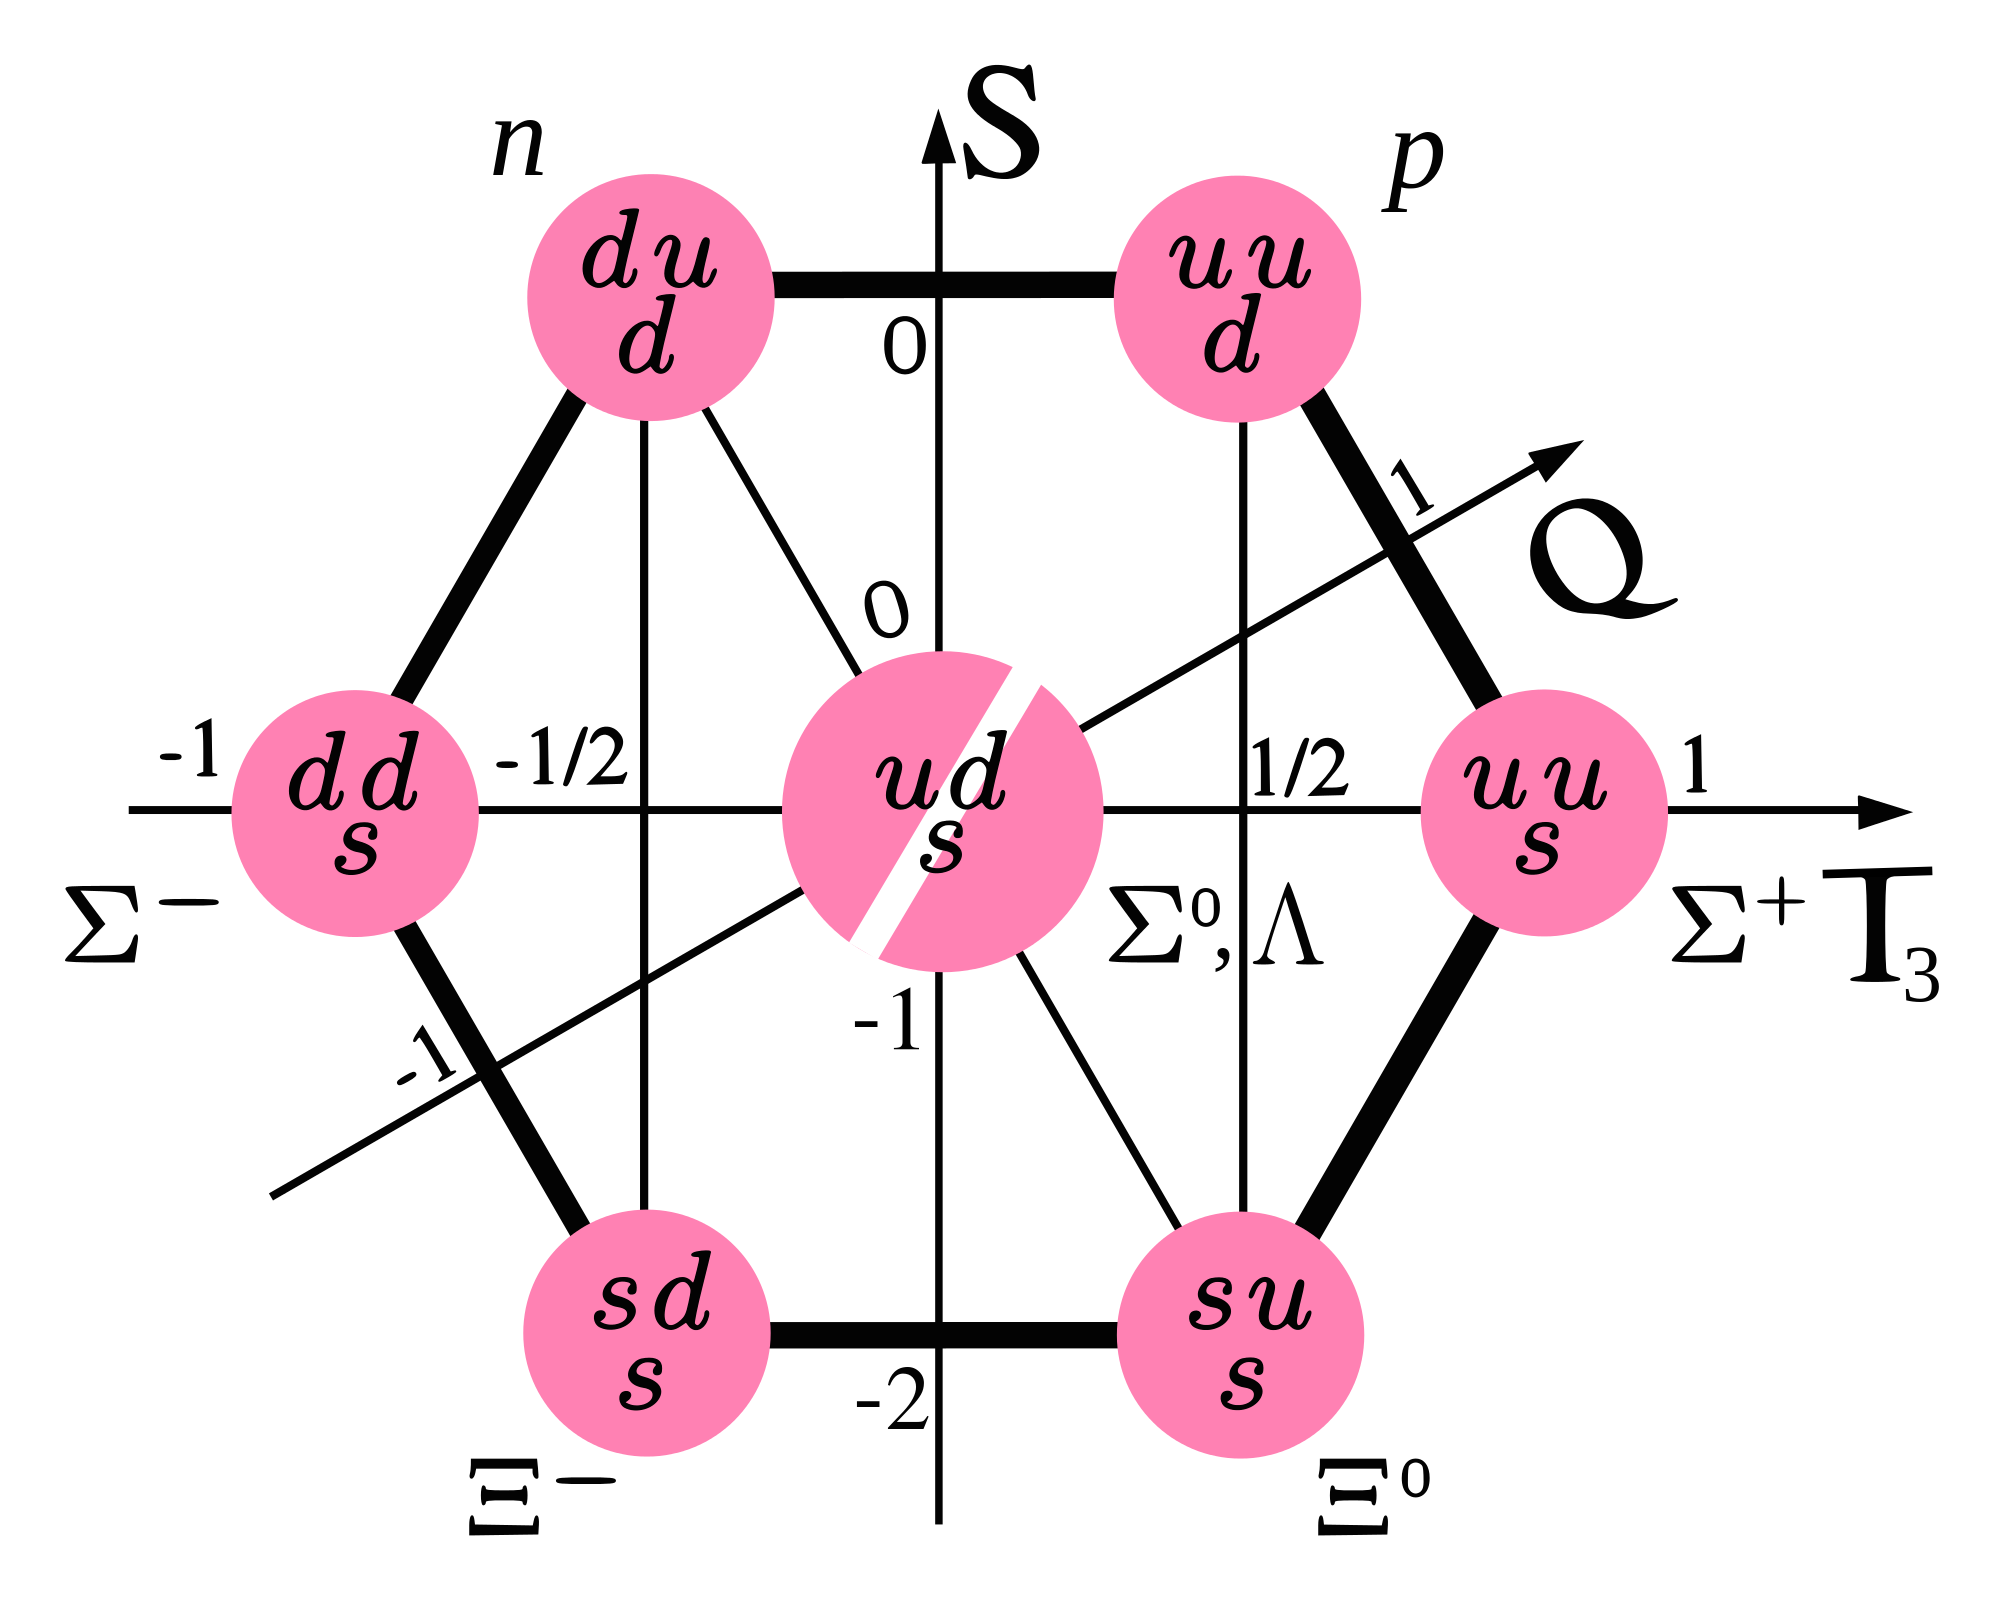
\includegraphics[width=0.6\textwidth]{Chapter1/Baryon-octet.png} 
  \caption{Baryonic octuplet encapsulating baryons from table
    \ref{tab:SelectedHadrons}. For baryons in this diagram, the relation $Y = S
    + 1$ holds. Figure from \cite{wiki:EightFoldWay}.}
  \label{fig:BaryonicOctet}
\end{SCfigure}

It is possible to find another representations of Lie algebra, to which the
observed hadrons can be assigned. The simplest way seems to be through highest
weight defining representation. From eigenvalues of adjoint representation
\eqref{eq:RepresentLie8} one can find simple roots 
$\alpha^1=\left( \frac{1}{2}, \frac{\sqrt{3}}{2} \right)$, 
$\alpha^2=\left( \frac{1}{2}, - \frac{\sqrt{3}}{2} \right)$, 
from which the highest weights follow
$\mu^1=\left( \frac{1}{2}, \frac{\sqrt{3}}{6} \right)$, 
$\mu^2=\left( \frac{1}{2}, - \frac{\sqrt{3}}{6} \right)$. 
New representation of Lie algebra can be constructed from highest weight. This
procedure is described in \cite{LieAlgebrasForParticlePhysicists} in detail.

Representations defined by highest weight $\mu^1$ or $\mu^2$ respectively are
called fundamental. Fundamental representation defined by $\mu^1$ is usually
denoted $\mathbf{3}$ and was encountered already by expressions
\eqref{eq:RepresentLie3} with weight diagram at Figure~\ref{fig:QuarkTriplet},
corresponding to three different quark states. The second fundamental
representation corresponds to three anti-quark states and is usually denoted
$\bar{\mathbf{3}}$. Representation depicted in Figure~\ref{fig:BaryonicOctet} is
defined by the highest weight $\mu^1 + \mu^2$.

Special interest is in representations with dimensions $10$ and $8$. These
are present in decompositions $\mathbf{3} \otimes \mathbf{3} \otimes
\mathbf{3} = \mathbf{10} \oplus \mathbf{8} \oplus \mathbf{8} \oplus \mathbf{1}$,
which correspond to the baryons composed of three quarks, and $\mathbf{3}
\otimes \bar{\mathbf{3}} = \mathbf{8} \oplus \mathbf{1}$ corresponding to
mesons from quark and anti-quark.

Important feature of quark model just presented is its capability to predict
hadron masses. This is done using Gell-Mann--Okubo mass formula
\cite{Gell-Mann:1250016,Okubo01051962}

\begin{equation}
  M = a_0 + a_1 S + a_2 \left( T(T+1) - \frac{1}{4}S^2 \right),
  \label{eq:GellMannOkubo}
\end{equation}
where $a_0$, $a_1$ and $a_2$ are free parameters which are common for all
hadrons in one multiplet. 

In 1970 Sheldon Lee Glashow, John Iliopoulos and Luciano Maiani proposed
\cite{Quarks4} an extension which predicted existence of fourth flavor of quark
- charm quark.
In 1973 the Makoto Kobayashi and Toshihide Moskawa proposed \cite{Quarks6} that the
existence of 6 different quark flavors could explain the experimental
observation of CP violation.


\section{Experimental Ground}

In the previous section it was shown the hadrons can be categorized using
representations of $\mathfrak{su}(3)$ Lie algebra. This lead to the model, where
baryons were composed of three quarks whereas the mesons of quark and
anti-quark. In this section, some experimental evidences will be presented to
support quark model. First the scattering reactions will be discussed. It will
be shown, that the lepton scattering on nucleons can be explained by assumption,
that nucleons are composed of point-like spin-1/2 particles. Next discussion
will address the fact, that there are three color charges - this will encounter
the question, why the group $SU(3)$ is connected to the theory of strong
interaction.

\subsection{Scattering Reactions}

One of the possibilities, how to find out, if there is some inner structure in
nucleon $N$, are the scattering reactions

\begin{align}
  &e^- \, (E \gg 1\GeV) + N \rightarrow e^- + N,
  \label{eq:ScatteringReactionsElectron} \\
  &\nu_e \,\, (E \gg 1\GeV) + N \rightarrow \nu_e + N,
  \label{eq:ScatteringReactionsNeutrino}
\end{align}
where the condition $E \gg 1 \GeV$ is explicitly written to ensure the wavelength
of lepton being $< 0.2\,\text{fm}$. By the first scattering reaction, the information
about electric charge distribution in nucleon can be extracted, whereas the
second scattering reaction informs us about weak charge distribution. Further only
\eqref{eq:ScatteringReactionsElectron} will be discussed. Feynmann diagram of this
process is depicted with kinematics variables and vertex algebraic structures 
in Figure~\ref{fig:Scattering}. 

\begin{SCfigure}
  \centering
  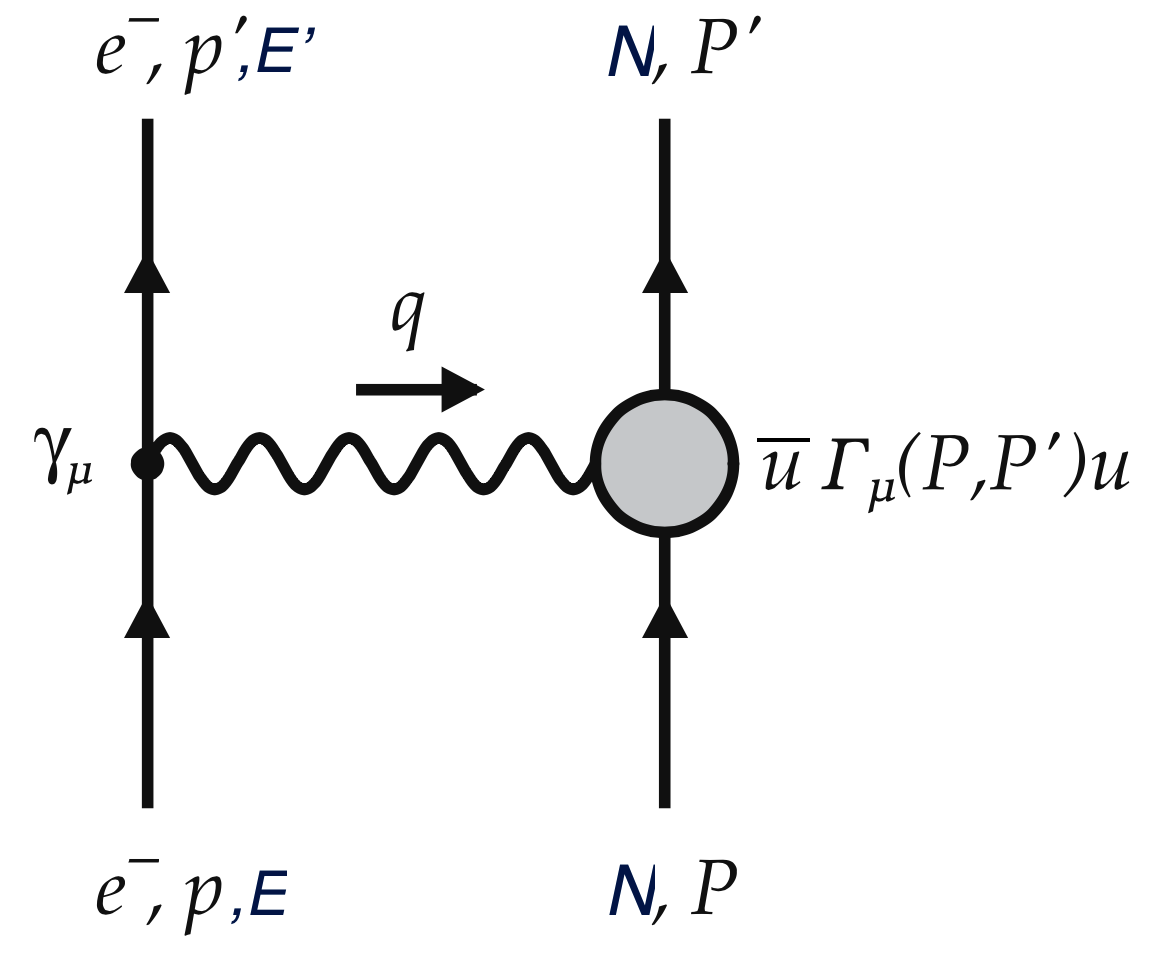
\includegraphics[width=0.6\textwidth]{Chapter1/Scattering.png} 
  \caption{Scattering reaction $e^-N \rightarrow e^-N$ with kinematics variables
    and algebraic structures of vertices. Figure from \cite{QCDTextbook}.}
  \label{fig:Scattering}
\end{SCfigure}

Because of Lorentz-invariance of Quantum Electrodynamics (QED), the matrix
element of the nucleon vertex $\bar{u}(P',S')\Gamma_\mu u(P,S)$ has to be a
Lorentz-vector. This restricts the possible form of $\Gamma_\mu$ to the
following algebraic structure

\begin{equation}
  \Gamma_\mu = A \gamma_\mu + B P_\mu' + C P_\mu + i D P'^\nu \sigma_{\mu\nu}
    + i E P^\nu \sigma_{\mu\nu},
  \label{eq:ScatteringAlgebraicMatrix}
\end{equation}
where $A$,\dots,$E$ depend only on Lorentz-invariant quantities. Next condition
which has to be taken into account, is gauge invariance of matrix element, which
can be written in the form

\begin{equation}
  q^\mu \bar{u}(P',S')\Gamma_\mu u(P,S).
  \label{eq:ScatteringGaugeInvariance}
\end{equation}

The further computation of cross section is straightforward and the result can
be easily generalized to non-elastic scattering by which the nucleon in final
state decays. The result is usually written using inelasticity parameter
$y=\frac{E-E'}{E}$, $0 \leq y \leq 1$, $y=0$ corresponding to the elastic
scattering, Bjorken variable $ x = \frac{Q^2}{2 P \cdot q}$, $ 0 < x \leq 1$, $x
= 1$ denoting elastic scattering and finally instead of negative value $q^2$ the
$Q^2 = -q^2$ is used. Final result can be than written in the form

\begin{equation}
  \left. \frac{d^2\sigma}{dxdy} \right|_{eN} =
  \frac{8 \pi M_N E \alpha^2}{Q^4} \left[ x y^2 F_1^{eN}(Q^2, x)
  + (1-y) F_2^{eN}(Q^2,x) \right].
  \label{eq:ScatteringRes1}
\end{equation}
The $eN$ sub(super)script stresses the fact, we are dealing with scattering
\eqref{eq:ScatteringReactionsElectron}. $F_1^{eN}$ and $F_2^{eN}$ are the so
called structure functions, which are not determinable by the theory just
presented - they have to be measured experimentally.

Structure constants were first measured by $eP$ scattering at SLAC in 1968
\cite{ePScattering} and shown the following results
\begin{enumerate}
  \item for $Q^2 \geq 1\GeV$, there is no significant dependence of structure
    functions on $Q^2$ and
  \item for $Q^2 \geq 1\GeV$, $F_2 \approx 2xF_1$.
\end{enumerate}
These results can be explained by assumption nucleon being composed of
point-like spin-1/2 constituents, for which R. P. Feynmann used the term partons. In
the following basic ideas of parton model will be presented. To $i$th parton, it
is possible to assign momentum $P_{i,\xi}$

\begin{equation}
  P_{i,\mu} = \xi_i P_\mu + \Delta P_{i,\mu} 
    \quad , \quad \max_\mu (\Delta P_\mu) \ll \max_\mu P_\mu,
  \label{PartonsMomentumDistriburtionAssumption}
\end{equation}
where $\xi_i \in \left< 0, 1 \right>$ and $\Delta P_{i,\mu}$ comes from the
interaction between partons and it is assumed, the momentum coming from this
interaction is much smaller than the total nucleon momentum $P_\mu$. In
addition, probabilities $f_i(\xi_i)$ that $i$th parton will carry $\xi_i$
fraction of total momentum fulfilling

\begin{equation}
  \int d\xi_i f_i(\xi_i) = 1
  \label{eq:PartonDensityFunctionsNormalization}
\end{equation}
must be defined. Then for scattering reaction
\eqref{eq:ScatteringReactionsElectron} the total cross section
formula can be derived

\begin{equation}
  \left. \frac{d^2\sigma}{dxdy} \right|_{eN} =
  \frac{4 \pi M_N E \alpha^2}{Q^4} \left[ y^2 + 2 ( 1 - y ) \right]
  \sum_i f_i(x) q_i^2 x.
  \label{eg:ScatteringRes2}
\end{equation}
where for $i$th parton its electrical charge $q_i$ was introduced. The last
expression and \eqref{eq:ScatteringRes1} can be compared as polynomials in $y$
resulting in

\begin{equation}
  F_1^{eN}(x) = \frac{1}{2} \sum_i f_i(x)q_i^2
  \quad , \quad
  F_2^{eN}(x) = \sum_i f_i(x) q_i^2 x.
  \label{eq:StructureFunctionAndPDF}
\end{equation}
It can be easily checked, that $F_2^{eN}(x) = 2 x F_1^{eN}(x)$. Functions
$f_i(x)$ just introduced are called Parton Distribution Functions (PDFs) and their
important role in QCD will be discussed in \ref{sec:ComaprisonWithNLOPrediction}
in more details.

Important conclusion from analyzing of scattering reactions is, that the
experimental results can be explained by assumption nucleons being composed of
spin-1/2 point-like partons, now called quarks. 

\subsection{Number of Colors}

Despite the strong confidence in the parton model, a theory which would describe the
interaction between partons was still missing. There was no direct evidence on
how the theory would look like at the beginning of 1970s. The theory of electroweak
unification successfully suggested, that the gauge theories are the right
theories for the description of our world at the subatomic level, but to construct gauge
theory of strong interaction the number of colors first had to be known.

Number of colors $N_C$ is the number of different kinds of quarks of the same
flavor with respect to the new interaction. In this part, three arguments will
be presented to demonstrate, that $N_C = 3$.

The first argument is the analysis of the electron-positron annihilation into the
pair of fermion and anti-fermion

\begin{equation}
  e^+e^- \rightarrow f\bar{f}.
  \label{ElectronPositronAnihilation}
\end{equation}

Feynmann diagram of this reaction is shown in Figure~\ref{fig:RRatio}, where
constants sitting in two vertices are emphasized.  $\alpha$ stands for fine
structure constants and $Q_f$ for charge of fermion $f$ in units of positron
charge. Total cross section has to be proportional to

\begin{figure}[h!]
  \centering
  \begin{subfigure}[b]{0.45\textwidth}
    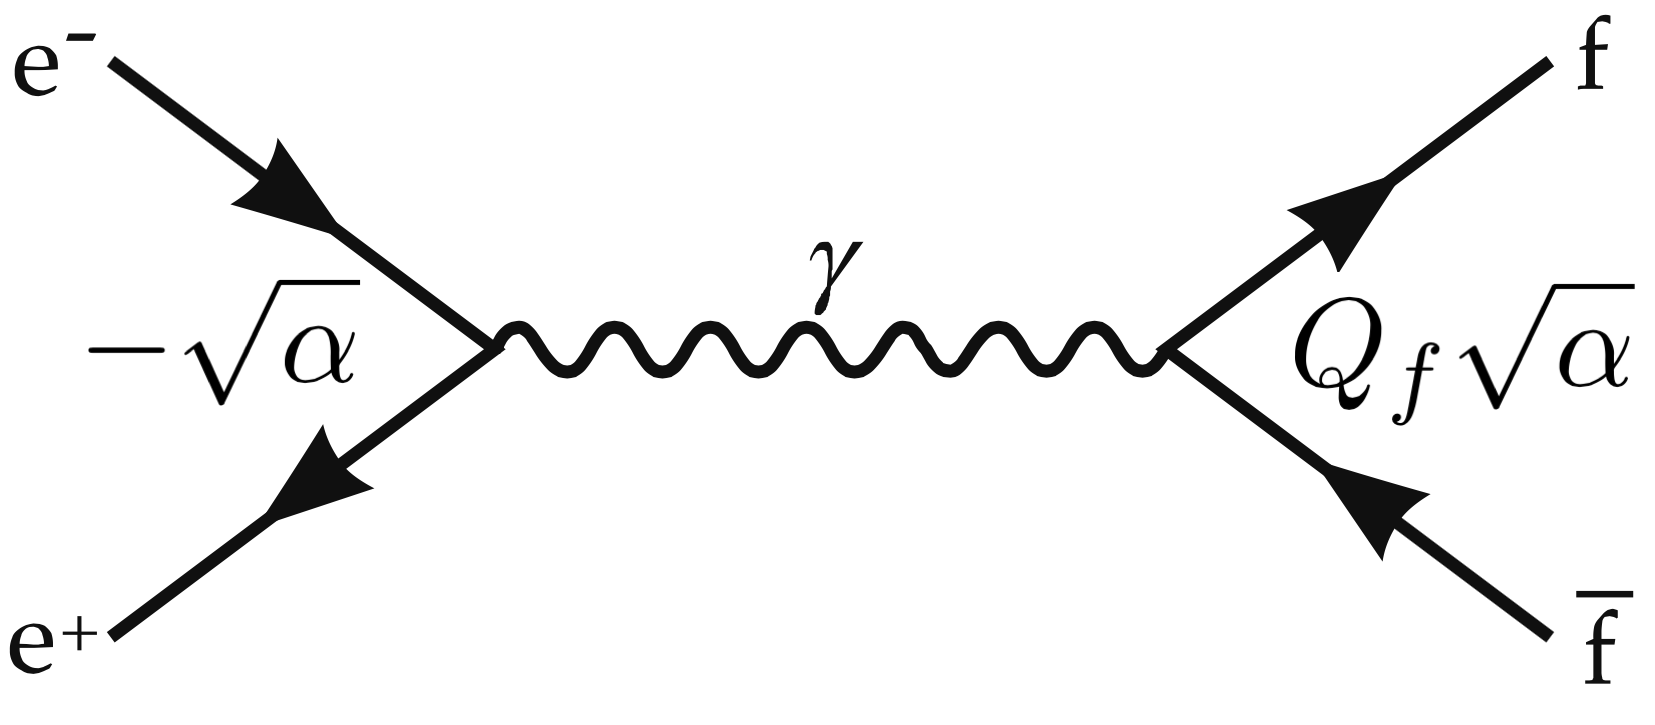
\includegraphics[width=\textwidth]{Chapter1/RRatio.png} 
    \caption{$e^+e^- \rightarrow f\bar{f}$}
    \label{fig:RRatio}
  \end{subfigure}
  \quad
  \begin{subfigure}[b]{0.45\textwidth}
    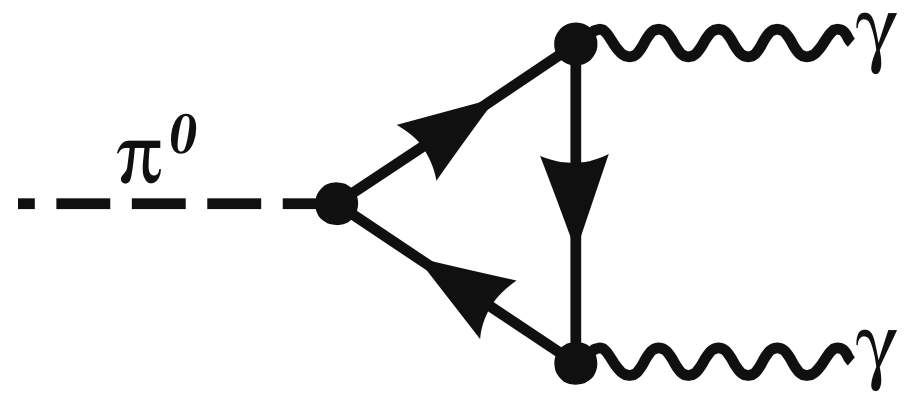
\includegraphics[width=\textwidth]{Chapter1/PiMesonDecay.png}
    \caption{$\pi^0 \rightarrow 2 \gamma$}
    \label{fig:PiDecay}
  \end{subfigure}
  \caption{(a) $e^-e^+$ annihilation into the pair of fermion anti-fermion.
    Constants siting in both vertices are dented with $\alpha$ being the fine
    structure constant and $Q_f$ the charge of fermion $f$ in units of positron
    charge.
           (b) $\pi^0$ meson decay into pair of photons with closed fermion
         loop.}
  \label{fig:FeynmannGraphsNC3}
\end{figure}

\begin{equation}
  \sigma (e^- e^+ \rightarrow f \bar{f} ) \sim Q_f^2 \alpha^2.
  \label{eq:NumberOfColorsBasicCrossSection}
\end{equation}
In the case fermion $f$ being quark, there is new degeneracy in final state
coming from different colors of quarks in final state - the total cross section
has to be multiplied by factor $N_C$. Experimentally, the so called $R$-factor
is measured

\begin{equation}
  R = \frac{\sigma(e^+ e^- \rightarrow \text{hadrons})}{\sigma(e^+ e^-
  \rightarrow \mu^+ \mu^-)} = \left( \sum_q Q_q^2 \right) N_C,
  \label{eq:NumberOfColorsRatio}
\end{equation}
where the sum on the left hand side is over all possible quark states. When the
quark model proposed by Gell-Mann a Zweig is used, then for the quark charges in
Table~\ref{tab:SelectedQuarks}

\begin{equation}
  R = \left[ \left( \frac{2}{3} \right)^2 +
    \left( \frac{-1}{3} \right)^2 +
  \left( \frac{-1}{3} \right)^2 \right] N_C = \frac{2}{3}N_C.
  \label{eq:NumberOfColorsSubstitued}
\end{equation}
Experimental results for $R$-ratio have shown \cite{PDG}, that $N_C = 3$.

The second argument is the measurement of decay width of $\pi_0$ meson. Decay is
depicted in Figure~\ref{fig:PiDecay}. For decay width $\Gamma$ it can be derived 

\begin{equation}
  \Gamma = 7.63 \left( \frac{N_C}{3} \right)^2 \, \text{eV},
  \label{ex:PiMesonDecayWidth}
\end{equation}
which, compared to the experimental value $\Gamma = 7.57 \pm 0.32 \, \text{eV}$
\cite{PDG}, leads again to $N_C=3$.

The third argument is purely theoretical and states, that the SM is internally
consistent only if there are three colors \cite{QCDTextbook}. This indicates that there
is some linking between electroweak and strong sector of SM and motivates the
search for Grand Unified Theories.

\section{QCD as a Gauge Theory}

Putting arguments of previous section all together, there is strong
experimental evidence, that nucleons consist of point-like spin-1/2 particles
called quarks and that quarks bring into the theory new degeneracy factor $N_C =
3$, which can be understood as three different strong charges called colors.

Nowadays the quark-quark strong interaction is understood as an $SU(3)$ gauge theory in
a degree of freedom called color. Gell-Mann matrices \eqref{eq:GellMannMatrices}
can be chosen as generators of $SU(3)$. These matrices act on quark color
triplets wave functions

\begin{equation}
  \psi(x) = \begin{pmatrix}  
    \psi_r(x) \\ \psi_g(x) \\ \psi_b(x) \\ 
            \end{pmatrix}.
  \label{eq:QuarkWaveFunction}
\end{equation}
Following the Yang-Mills theory \cite{YangMill}, to each generator
$\frac{\lambda^a}{2}$ gluon field $A_\mu^a(x)$ and gluon field strength tensor

\begin{equation}
  F_{\mu\nu}^a = \left( \partial_\mu A_\nu^a - \partial_\nu A_\mu^a + g f^{abc}
  A_\mu^b A_\nu^c \right)
  \label{eq:GluonFieldStrengthTensor}
\end{equation}
is assigned where $g$ denotes the coupling constant of strong interaction and
$f^{abc}$ are structure constant defined in section~\ref{Sec:TheoreticalAnsatz}.
QCD Lagrangian

\begin{equation}
  \mathscr{L}_{\text{QCD}} = \bar{\psi} \left( -i \partial_\mu + g \frac{\lambda}{2}
  A_\mu^a(x) \right) \gamma^\mu \psi - \frac{1}{4}F_{\mu\nu}^aF_a^{\mu\nu}
  \label{eq:QCDLagrangian}
\end{equation}
is invariant under local transformation

\begin{align}
  &\psi(x) \, \, \, \rightarrow \psi'(x) = \Euler^{ig\Theta(x)} \psi(x),
    \label{eq:QCDGaugeTranform} \\
  &A_\mu(x) \rightarrow \Euler^{ig\Theta(x)} \left( A_\mu(x) +
    \frac{i}{g}\partial_\mu \right) \Euler^{-ig\Theta(x)}, 
  \nonumber
\end{align}
where

\begin{equation}
  \Theta(x) = \frac{1}{2} \lambda^a \Theta^a(x) 
  \quad , \quad
  A_\mu(x) = \frac{1}{2} \lambda^a A_\mu^a(x).
  \label{eq:QCDAdditionalFunctions}
\end{equation}

There is no mass term in Lagrangian \eqref{eq:QCDLagrangian} because mass term
$m\bar{\psi}\psi$ vary under gauge transformation
\eqref{eq:QCDGaugeTranform}. Origin of mass term lies in Higgs mechanism
\cite{HiggsMechanism} which is explained in \cite{horejsi2002fundamentals} in
details.

QCD Lagrangian \eqref{eq:QCDLagrangian} together with gauge transformations
\eqref{eq:QCDGaugeTranform} are sufficient for determination of Feynman rules -
key ingredient in perturbative QCD which will be discussed in next section.

By derivation of gluon propagator, one has to add to the QCD Lagrangain the so
called gauge-fixing term

\begin{equation}
  \mathscr{L}_{\text{QCD}}^{\text{gauge-fixing}} = - \frac{1}{2\xi} \left( \partial_\mu A_a^\mu
  \right)^2,
  \label{eq:QCDGaugeFixingTerm}
\end{equation}
which confines the possible gauges to one class parametrized by real parameter
$\xi$. In non-Abelian gauge theories this term must be supplemented by the so
called ghost term which brings into the theory new unphysical scalar particle
obeying fermionic statistics. More details on so called Faddev-Popov ghost field
can be found in \cite{FaddeevPopovGhosts}.


\section{Perturbative QCD}

Quantum Electrodynamics (QED) and QCD are both quantum filed gauge theories, but
they differ in one killing feature - the former is Abelian whereas the latter is
not. The non-Abelian character of QCD leads to new phenomenons which have the origin in QCD
Lagrangian \eqref{eq:QCDLagrangian} directly leading to triple and quartic
gluonic interactions. In this section one remarkable consequence will be
discussed - the running coupling constant.

Assume scattering process  

\begin{equation}
  q \bar{q} \rightarrow q \bar{q},
  \label{eq:QuarkScattering}
\end{equation}
which is depicted in the lowest order of perturbation theory by the Feynman
graph in Figure~\ref{fig:QuarkQuarkScattering}. Except contribution of this
graph to the scattering amplitude (which is the only contribution $\sim g^2$)
there are 12 other Feynman diagrams with contributions $\sim g^4$. These are
depicted in Figure~\ref{fig:QuarkQuarkScatteringCorrection}. 

\begin{SCfigure}
  \centering
  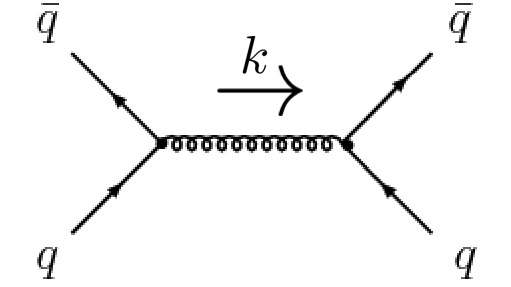
\includegraphics[width=0.5\textwidth]{Chapter1/QuarkQuarkScattering.png} 
  \caption{Leading order Feynmann diagrams in scattering reaction $q \bar{q}
    \rightarrow q \bar{q}$ with denoted transfered momentum $k$.}
  \label{fig:QuarkQuarkScattering}
\end{SCfigure}

\begin{figure}[t]
  \centering
  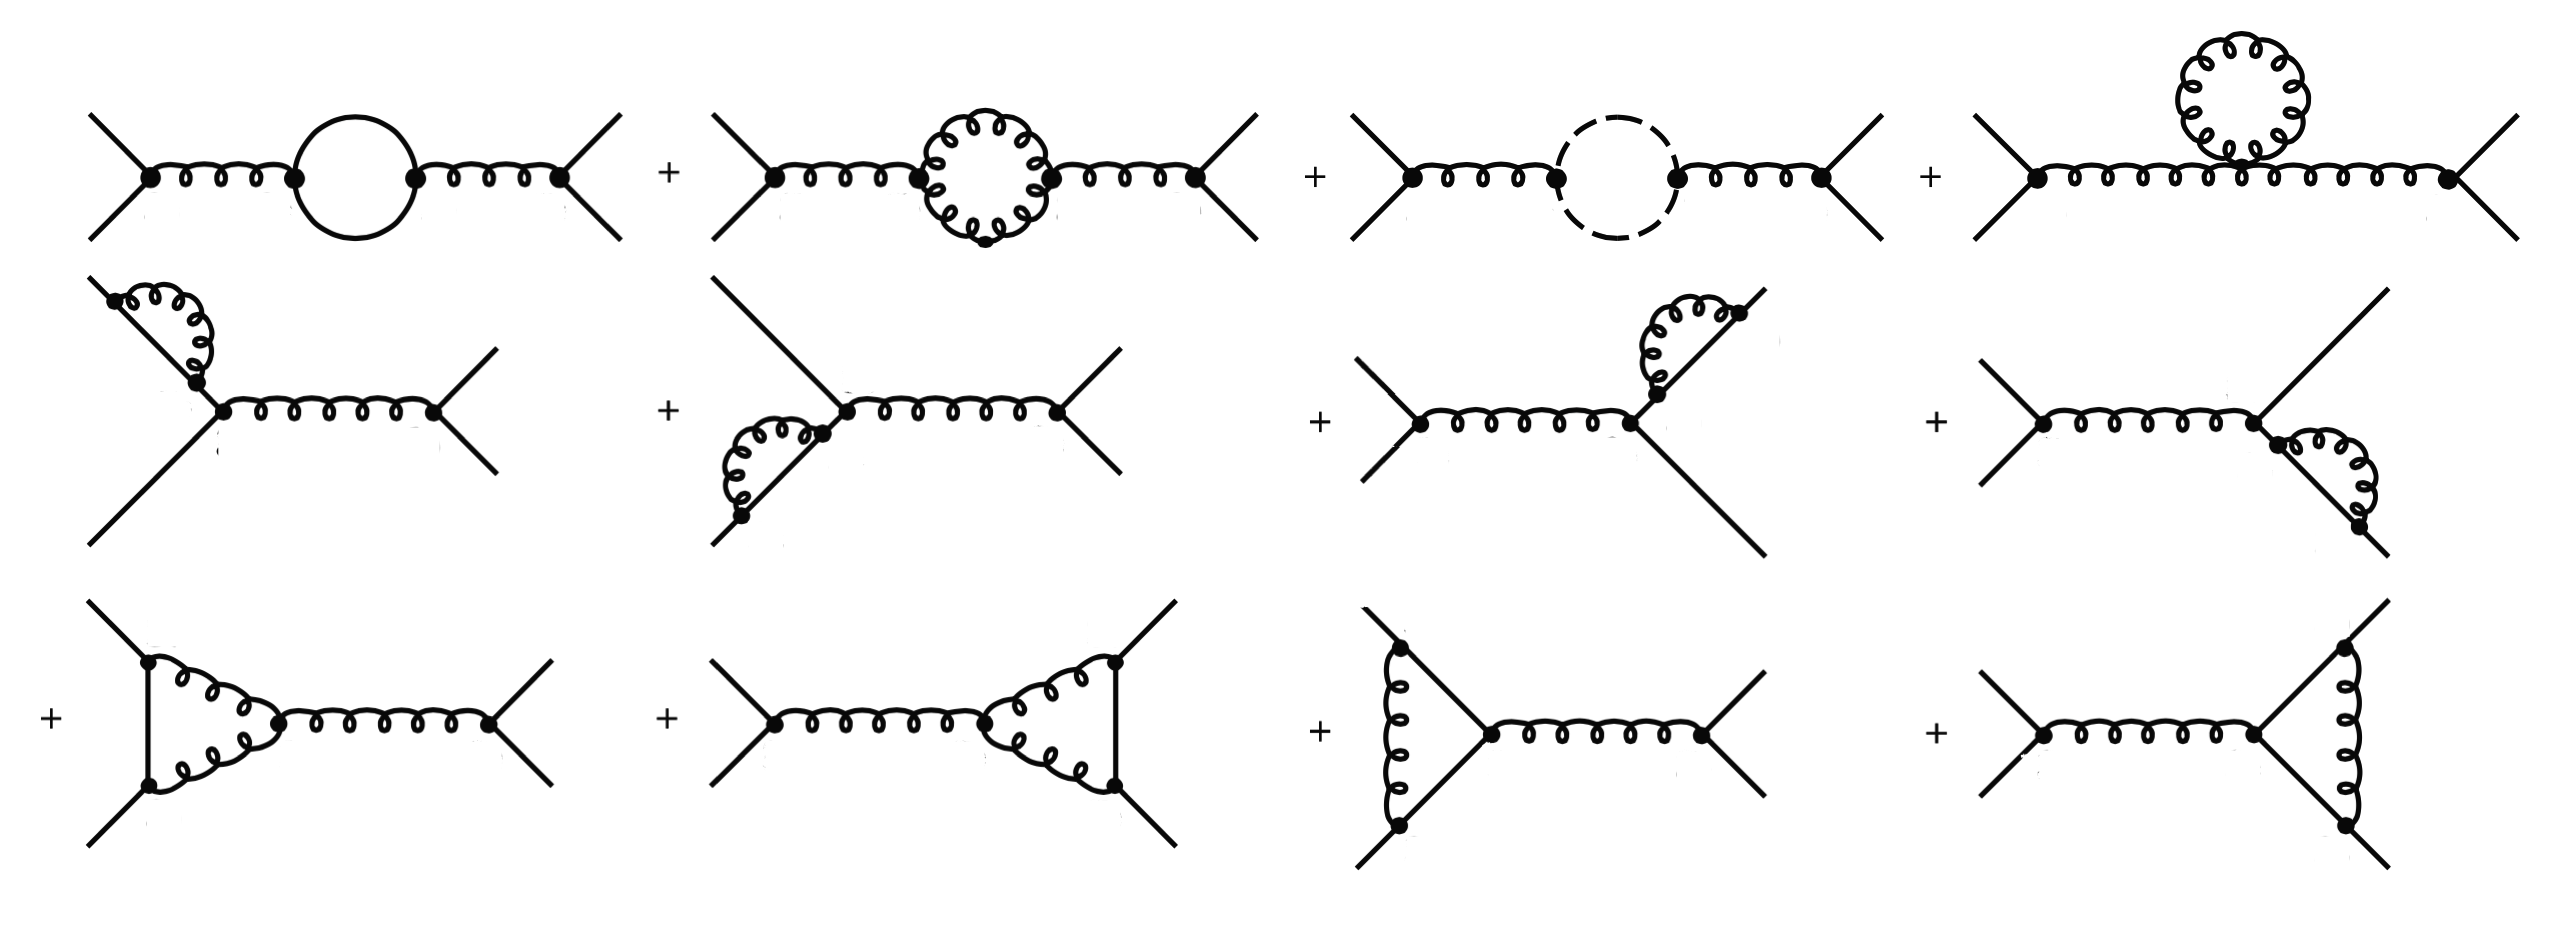
\includegraphics[width=\textwidth]{Chapter1/QuarkQuarkCorrection.png} 
  \caption{Next to the leading order Feynmann diagrams in scattering reaction
    $q \bar{q} \rightarrow q \bar{q}$. Dashed line represents scalar ghost
  particle.}
  \label{fig:QuarkQuarkScatteringCorrection}
\end{figure}

The contributions from new Feynman diagrams are calculated in \cite{QCDTextbook}
in detail. There is shown, that all this contributions together are
logarithmically divergent. This divergence can be removed, when from the scattering
amplitude for arbitrary momentum transfer $k^2$ scattering amplitude for fixed
momentum transfer $k^2 = -M^2$ is subtracted. This is how the renormalized
coupling constant $g_R$ is obtained and here is its final expression 

\begin{equation}
  g_R = g_0 - \frac{g_0^3}{16\pi^2} \left( \frac{11}{2} - \frac{1}{3}N_F \right)
  \ln \left( \frac{-k^2}{M^2} \right) + \mathscr{O}(g_0^5).
  \label{eq:RenormalizedCoupling}
\end{equation}
Here $g_0$ stands for the coupling constant measured at the renormalization scale
$k^2 = -M^2$ and $N_F$ is the number of different quark flavors with mass $m^2
\ll \left| k^2 \right|$. Dependence of $g_R$ on transfered momentum $k^2$ is
evident, but there are another two intertwined dependences - on normalization
scale $M$ and on coupling constant at renormalization scale $g_0 =
\left. g_R \right|_{k^2=-M^2}$. For next purpose, it is convenient to use the
dependence schema

\begin{equation}
  g_R = g_R(-k^2,g_0(M))
  \label{eq:RunningCouplingConstantDependenceSchema}
\end{equation}
which allows the use of advantages of $\beta$-function and with the usage of the
equation \eqref{eq:RenormalizedCoupling}, the differential equation for $g_0(M)$
can be obtained

\begin{align}
  \beta(g_0) \equiv M \left( \frac{\partial g_R}{\partial M} \right)_{-k^2=M^2}
  &= M \left( \frac{dg_0}{dM} \right)_{-k^2=M^2}
  \label{eq:BetaFunction1} \\
  &= -b_0 g_0^3 + \mathscr{O}(g_0^5)
  , \quad b_0 = \frac{1}{16\pi^2}\left(11-\frac{2N_F}{3}\right),
  \label{eq:BetaFunction2}
\end{align}
which can be solved directly to obtain coupling constant $g_0$ for arbitrary
scale $-k^2$

\begin{equation}
  \int_{g_0(M^2)}^{g_0(-k^2)} \frac{dg_0}{g_0^3} =
  -b_0 \int_{M^2}^{-k^2}\frac{dM}{M}
  \label{eq:RunningCouplingConstantIntegralEquation}
\end{equation}
with solution

\begin{equation}
  \alpha_S(-k^2) = \frac{\alpha_S(M^2)}{1 + \frac{\alpha_S(M^2)}{4\pi} \left(
  11-\frac{2N_F}{3} \right) \ln \left( \frac{-k^2}{M^2} \right) }
  , \quad g_0^2(-k^2) = 4 \pi \alpha_S( -k^2 ),
  \label{eq:RunningCouplingConstant}
\end{equation}
which is the final expression for running coupling constant up to one-loop
order. This dependence corresponds to experimental data which are depicted in
Figure \ref{fig:RunningCouplingConstant}. Coupling constant decreases with
increasing momentum transfer allowing the use of the perturbation theory. This
is known as Asymptotic Freedom \cite{AssymptoticFreedom}.

\begin{figure}[t]
  \centering
  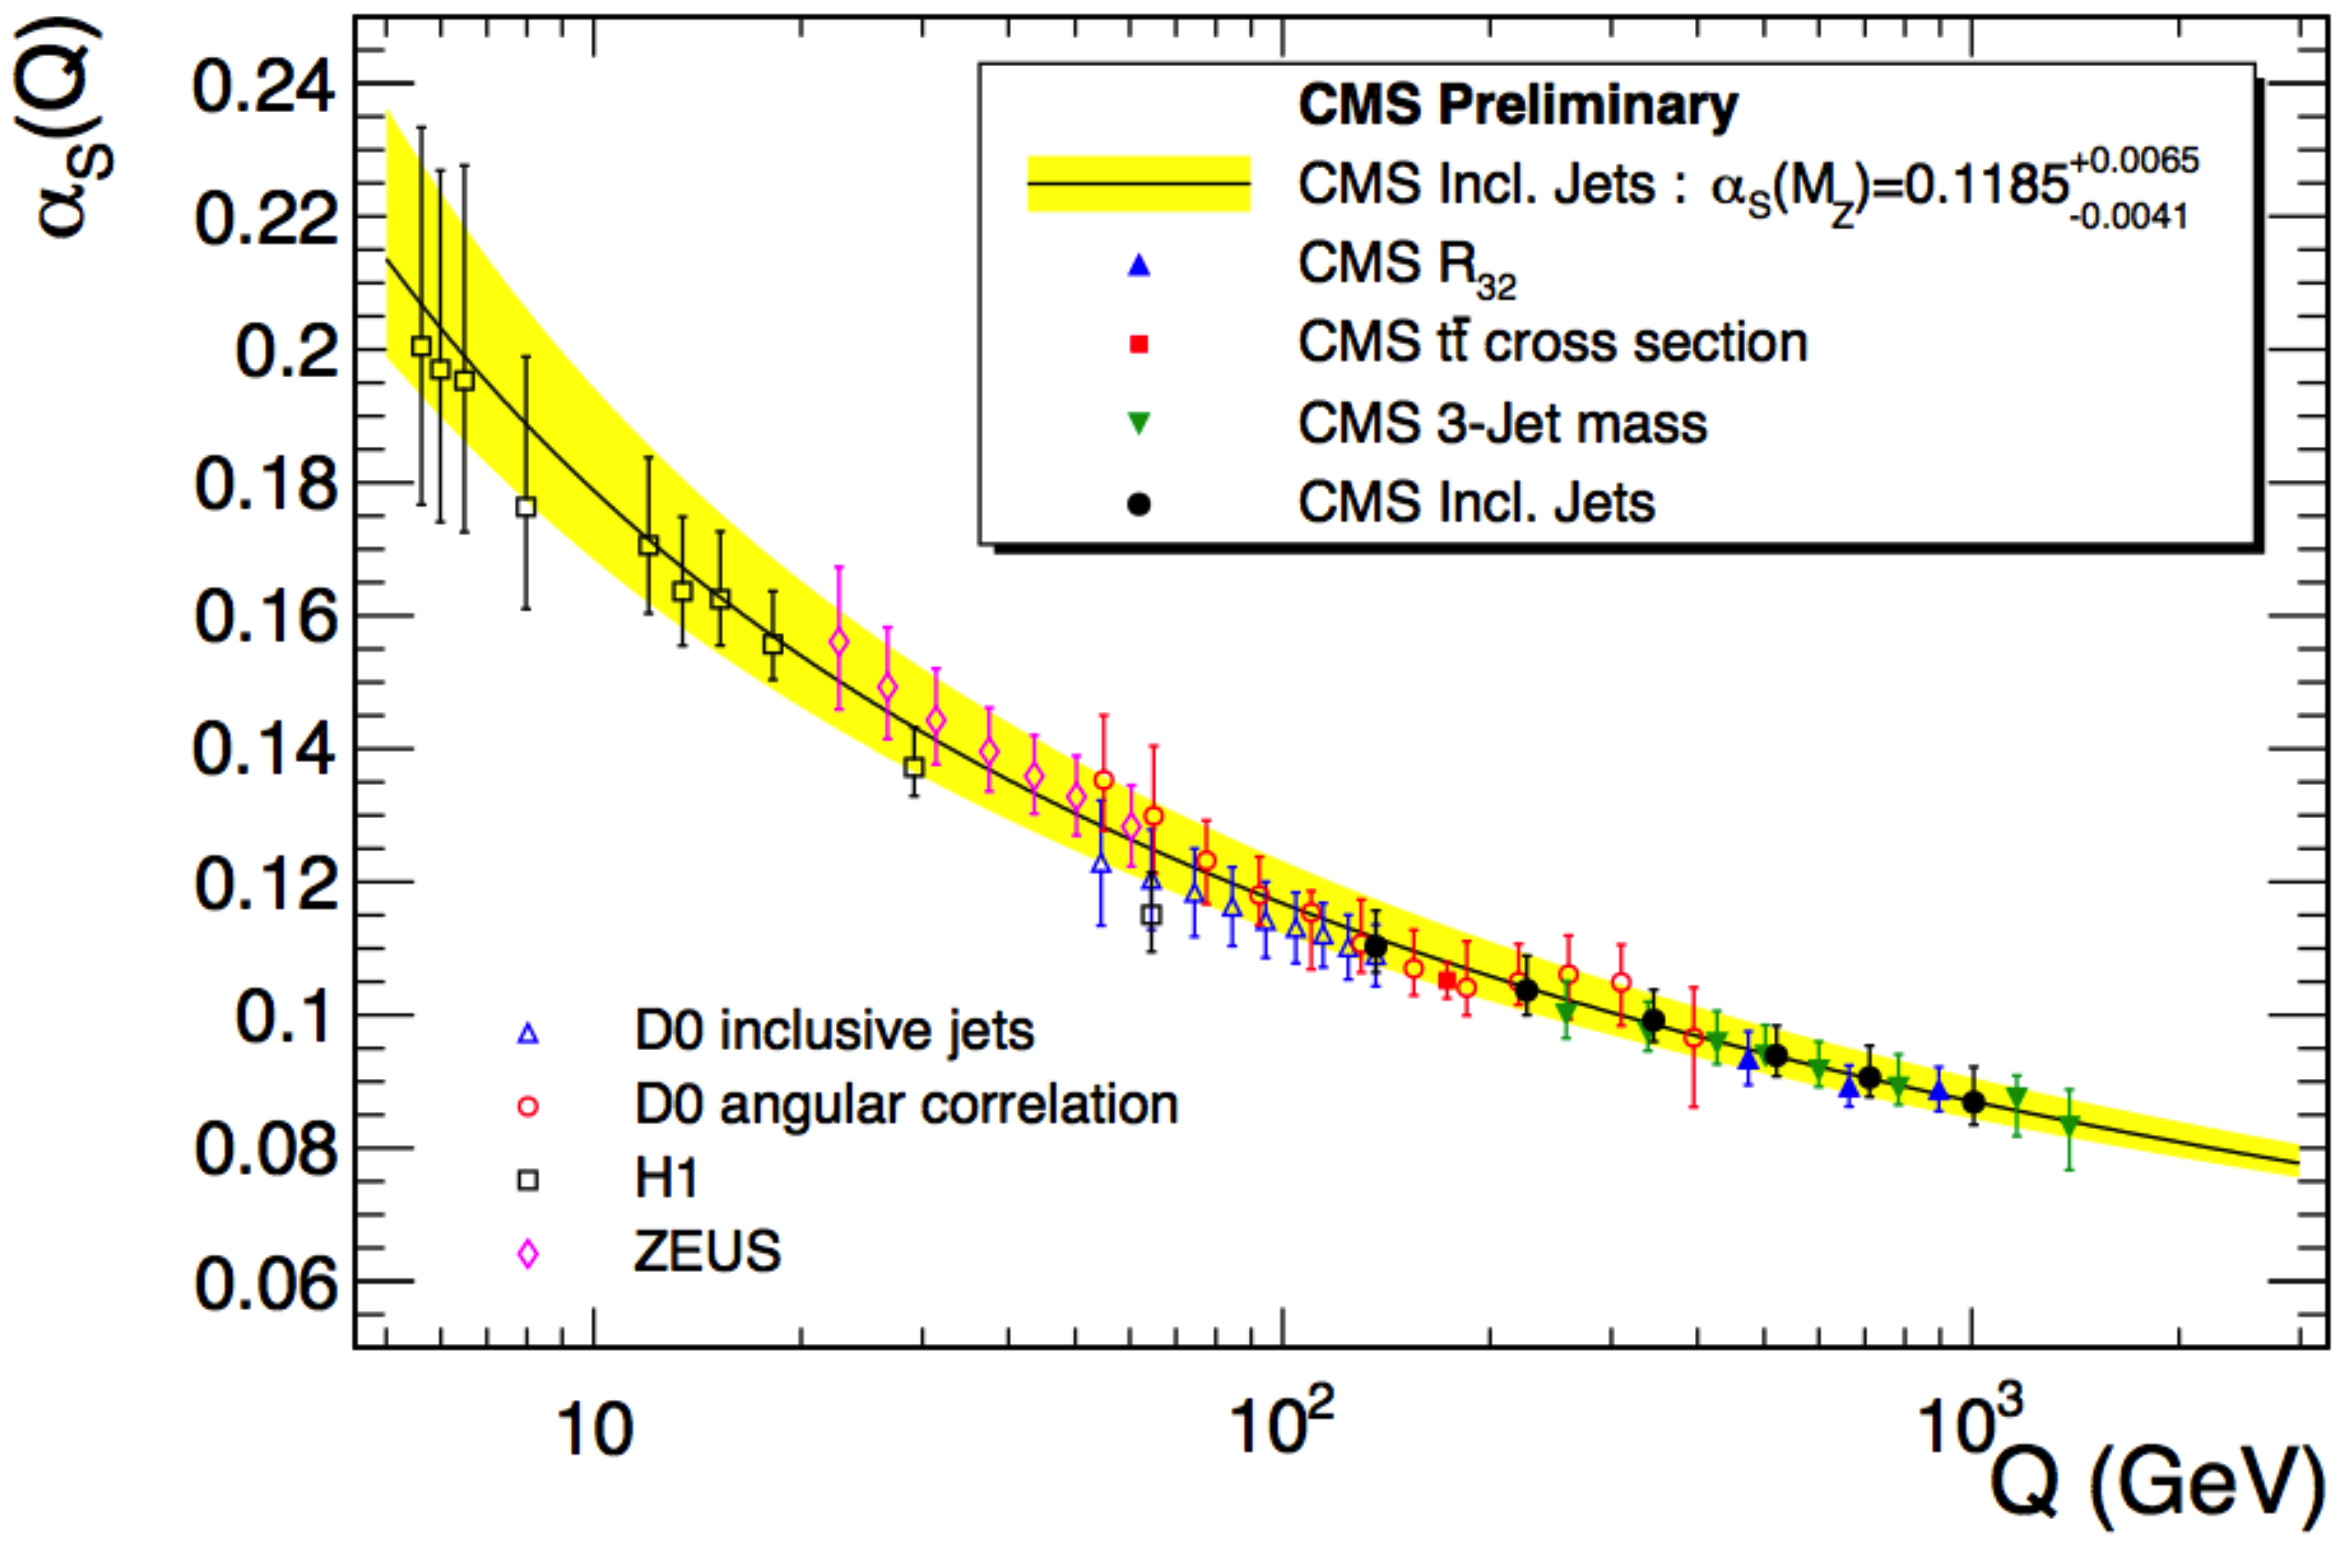
\includegraphics[width=0.8\textwidth]{Chapter1/RunningCouplingConstant.png}
  \caption{Experimental measurements of running coupling constant $\alpha_S(Q)$
    (solid line) and its uncertainty (yellow band).
    $Q=\sqrt{\left|k^2\right|}$ in comparison to
    \eqref{eq:RunningCouplingConstant}. Figure from
    \cite{RunningCouplingConstantMess}. }
  \label{fig:RunningCouplingConstant}
\end{figure}

On the other hand, when the momentum transfer decreases, there is special value
$-k^2=\Lambda^2$ for which the last expression diverges

\begin{equation}
  -1 = \frac{\alpha_S(M^2)}{4\pi} \left( 11 - \frac{2N_F}{3} \right)
  \ln \left( \frac{\Lambda^2}{M^2} \right).
  \label{eq:RunningLambda}
\end{equation}
Experimental value is $\Lambda=213^{+38}_{-35}\MeV$ \cite{wiki:QCDHistory} and demonstrates, that
perturbative QCD cannot be used at low energy transfers. In fact, the running
coupling constant $\alpha_S(-k^2)$ reaches value $\sim 1$ on momenta
transfers $\sqrt{\left| k^2 \right|} \sim 500\MeV$. 

The behaviour of coupling constant at low energy transfers is not explainable in
the language of perturpative QCD just presented. It is non-perturbative effect
known as the principle of color confinment, which states, that quarks when
seperate, the gluon force field between them becomes stronger and its energy is
consumed by the creation of quark anti-quark pair. This continues until there is
no free color charge left. This principle forbids us from observing free quarks.

To understand e.g. structure of proton with rest mass $< 1\GeV$ it is clear
non-perturbative QCD has to be used. The ideas of non-perturbative QCD will be
introduced in next section. 

\section{Non-Perturbative QCD}

The most well established non-perturbative approach to QCD is the lattice QCD
(LQCD). In this section basic features of the LQCD will be presented.  More
informations on this extended topic can be found in \cite{QCDTextbook,LQCDIntro}.

LQCD is QCD formulated on a hypercubic equally spaced lattice in space and time
with lattice parameter $a$ denoting the distance between neighboring sites.
Quark fields are placed on sites whereas the gluon fields sit on the links
between neighboring sites. From QCD it inherits the gauge invariance which has
to be formulated on lattice structure.  For $a \rightarrow 0$ action of LQCD
coincides with that of QCD. LQCD contains 6 parameters - strong coupling
constant and masses of 5 quarks (the top quark with lifetime $ \sim
10^{-24}\,\text{s}$ is not assumed by the theory).

Unlike perturbative expansion used in continuous QCD, numerical evaluation of
the path integral defining LQCD allows non-perturbative calculations.  Practical
LQCD calculations are limited by the availability of computational resources and
the efficiency of algorithms. LQCD suffers with both statistical and systematic
errors, the former arising from the use of Monte-Carlo integration, the latter,
e.g. from the use of non-zero values of $a$.

Present LQCD calculations are made on supercomputers like the QCDCQ
supercomputer \cite{SuperComputer} with peak speed of 500 TFlops using lattice
spacing $a \sim 0.05 - 0.15 \, \text{fm}$ in lattice volume $V \sim (2 - 6
\,\text{fm} )^3$.

The Importance of LQCD lies in its ability to predict mass spectrum of observed
mesons and baryons, including quark masses itself, and in investigation of
topological structure of QCD vacuum.  LQCD can be used to obtain PDFs
\eqref{eq:PartonDensityFunctionsNormalization} helping us to understand the
structure of hadrons. Phenomenology of LQCD explains also the principle of color
confinment. 


